
%(BEGIN_QUESTION)
% Copyright 2014, Tony R. Kuphaldt, released under the Creative Commons Attribution License (v 1.0)
% This means you may do almost anything with this work of mine, so long as you give me proper credit

Calculate the source voltage in this AC circuit, as well as the phase shift between source voltage and source current, given the voltage drops shown in the schematic diagram.  You may express the source voltage as a scalar number (i.e. no need to use rectangular or polar notation):

$$\includegraphics[width=15.5cm]{i01099x01.eps}$$

$V_{source}$ = \hskip 100pt $\theta$ = \hskip 100pt $V$ {\it leads} $I$ or $I$ {\it leads} $V$? 

\vskip 10pt

\underbar{file i01099}
%(END_QUESTION)





%(BEGIN_ANSWER)

$V_{source}$ = 7.151 V \hskip 100pt $\theta$ = 42.17$^{o}$ \hskip 100pt $V$ {\bf leads} $I$ 

%(END_ANSWER)





%(BEGIN_NOTES)

{\bf This question is intended for exams only and not worksheets!}.

%(END_NOTES)


